%********************************************************************************************
%								COMANDOS ÚTILES PARA LATEX EN ESTE TP							
%
%	\ : espacio simple
%	\\ : nueva línea
%	\par : va a la línea de abajo y deja sangría
%	\vspace{##tamaño en pt##} o \vspace{\baselineskip} en general:
%								 para dejar un espacio vertical
%	\textbf{text} :text en negrita
%	\textit{text} :text en itálica
%
% GRAFICOS CENTRADOS:
%	\begin{center}
%		\includegraphics[width=\textwidth]{./img/##ruta imagen (no hace falta extension)##}
%	\end{center}
%		--> se pueden agregar atributos como scale por si se hace muy grande
%
% TABLAS CENTRADAS:
%	\begin{center}
%	\begin{tabular}{|c|c|}
%	\hline
%	\ \textbf{Programa} & \textbf{Ticks} \\
%	\hline
%		ASM & 675127609 \\
%	\hline
%	\end{tabular}
%	\end{center}
%
% ALGORITMOS (EN VARIOS LENGUAJES):
% \begin{lstlisting}
%	void sumoDiez(int &num)
%	{
%	    num += 10;
%	}
%	
%	int main()
%	{
% 	   int i;
%	    int numeroAProcesar = 20;
%	    for (i = 0; i < 50; i++)
%	    {
%	        sumoDiez(numeroAProcesar);	//Proceso el numero en cada ciclo
%	    } 
%	    return 0;
%	}
%	\end{lstlisting}
%
% para info sobre todo lo que tiene el package detallado:
% http://en.wikibooks.org/wiki/LaTeX/Source\_Code\_Listings
%
%********************************************************************************************

\documentclass[10pt,a4paper]{article}
\usepackage[utf8]{inputenc} % para poder usar tildes en archivos UTF-8
\usepackage[spanish]{babel} % para que comandos como \today den el resultado en castellano
\usepackage{a4wide} % márgenes un poco más anchos que lo usual
\usepackage[conEntregas]{caratula}
\usepackage{amssymb}
\usepackage{fancybox}
\usepackage[usenames,dvipsnames]{color}
\usepackage{hyperref}
\usepackage{listings}
\usepackage{xcolor}
\usepackage{amsmath}

\hypersetup{
    colorlinks,
    citecolor=black,
    filecolor=black,
    linkcolor=black,
    urlcolor=black
}

\lstdefinestyle{customc}{
  belowcaptionskip=1\baselineskip,
  breaklines=true,
  frame=L,
  xleftmargin=\parindent,
  language=C,
  showstringspaces=false,
  basicstyle=\footnotesize\ttfamily,
  keywordstyle=\bfseries\color{green!40!black},
  commentstyle=\itshape\color{purple!40!black},
  identifierstyle=\color{blue},
  stringstyle=\color{orange},
}

\lstset{escapechar=@,style=customc}

\begin{document}

\titulo{Trabajo Práctico 1}
\subtitulo{Análisis preliminar del sistema de software “TecnoTaxi”}

\fecha{\today}

\materia{Ingeniería del Software I}
\grupo{}

\integrante{Barbeito, Nicolás}{LLL/AA}{nicolasbarbeiton@gmail.com}
\integrante{Chapresto, Matías}{LLL/AA}{matiaschapresto@gmail.com}
\integrante{Garassino, Agustín Javier}{394/12}{ajgarassino@gmail.com}
\integrante{Sarriés, Ana}{LLL/AA}{anasarries@yahoo.com.ar}
\integrante{Vileriño, Silvio}{LLL/AA}{svilerino@gmail.com}

\maketitle

\tableofcontents
\newpage

\section{Descripción general del sistema}
El objetivo del sistema es automatizar las solicitudes de taxis por parte de los pasajeros y la coordinación de los viajes con los taxistas. Para lograr esto se desarrollará una aplicación web, con la cual interactuarán tanto los clientes como los empleados de la empresa de RadioTaxi. Los pasajeros podrán comunicarse a través de internet para solicitar los viajes ya sea utilizando un dispositivo móvil o una computadora de escritorio. Tendrán la opción de elegir dentro de un listado de perfiles de choferes con información sobre: el modelo del auto, puntuación asiganda según antiguos pasajeros, etc. A su vez los taxistas interactuarán con el sistema utilizando dispositivos móviles que serán proveídos por la empresa de RadioTaxi, ellos tendrán un listado de posibles viajes a realizar, pudiendo aceptar uno de ellos en cualquier momento. Además, con el fin de mejorar el servicio, información sobre la ubicación de los taxis será obtenida a través de un dispositivo de posicionamiento global que se comunicará con el servidor web.

\vspace{\baselineskip}
        \begin{center}
		    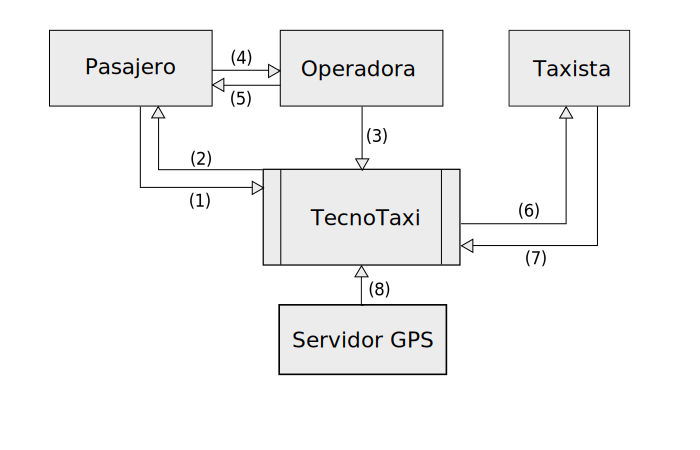
\includegraphics[scale=0.60]{contexto.jpeg}
		    \\
		    \vspace{1pt}
		    \footnotesize\textit{Diagrama de contexto del sistema “TecnoTaxi”.}
	    \end{center}
    \vspace{\baselineskip}
\par 
\newpage

\end{document}